%%
%% static_code_analysis_in_ci.tex
%% V0.1
%% 2015/01/22
%% by 
%% Sebastian Funke
%% Hamza Zulfiqar
%% Brian Pfretzschner
%% See:
%% https://github.com/hzulfiqar/SecSoftDev
%% for current contact information.
%%


\documentclass[conference]{IEEEtran}


% *** PACKAGES ***
%\usepackage{algorithmic}
%\usepackage{array}
%\usepackage{mdwmath}
%\usepackage{mdwtab}
%\usepackage{eqparbox}
%\usepackage{fixltx2e}
%\usepackage{stfloats}
\usepackage{cite}       % http://www.ctan.org/tex-archive/macros/latex/contrib/supported/cite/
\ifx\pdfoutput\undefined
\usepackage{graphicx}   % http://www.ctan.org/tex-archive/macros/latex/required/graphics/
\else
\usepackage[pdftex]{graphicx}
\fi
\usepackage{subfigure}  % http://www.ctan.org/tex-archive/macros/latex/contrib/supported/subfigure/
\usepackage{url}        % http://www.ctan.org/tex-archive/macros/latex/contrib/other/misc/
\usepackage[cmex10]{amsmath}    % http://www.ctan.org/tex-archive/macros/latex/required/amslatex/math/
%\usepackage{amsfonts}
\interdisplaylinepenalty=2500
\ifx\pdfoutput\undefined
\usepackage[hypertex]{hyperref}
\else                   % http://www.ctan.org/tex-archive/macros/latex/contrib/supported/hyperref/
\usepackage[pdftex,hypertexnames=false]{hyperref}
\fi
\usepackage[colorinlistoftodos,prependcaption,textsize=tiny]{todonotes}
\usepackage{listings}
\lstset{frame=single,captionpos=b}

% correct bad hyphenation here
\hyphenation{op-tical net-works semi-conduc-tor}

\begin{document}
%
% paper title
\title{An Evaluation of Open Source Static Code Analysis Reporting in Context of Continuous Integration Tools}



%\author{\IEEEauthorblockN{Sebastian Funke}
%\IEEEauthorblockA{Secure Software Engineering\\
%TU Darmstadt\\
%sebastian.funke@stud.tu-darmstadt.de}
%\and
%\IEEEauthorblockN{Brian Pfretzschner}
%\IEEEauthorblockA{Secure Software Engineering\\
%TU Darmstadt\\
%brian.pfretzschner@stud.tu-darmstadt.de}
%\and
%\IEEEauthorblockN{Hamza Zulfiqar}
%\IEEEauthorblockA{Secure Software Engineering\\
%TU Darmstadt\\
%hamza.zulfiqar@stud.tu-darmstadt.de}}



\author{\authorblockA{Sebastian Funke, Brian Pfretzschner, Hamza Zulfiqar}
	\authorblockA{Center for Advanced Security Research Darmstadt\\
		Department of Computer Science\\
		Technische Universit\"at Darmstadt, Germany}}




% use for special paper notices
%\IEEEspecialpapernotice{(Invited Paper)}




% make the title area
\maketitle


\begin{abstract}
Static code analysis should run frequently in an continuous integration lifecycle. Each run produces lots of information that need to be reviewed, evaluated and integrated in the ongoing development process. Therefore, the analysis results should be reported in a clear and meaningful fashion. Additionally, results might be combined, reworked, concentrated or filtered. We use only open source tools that a freely available and examine how they work together and what their results look like.
\end{abstract}

% no keywords

% For peerreview papers, this IEEEtran command inserts a page break and
% creates the second title. It will be ignored for other modes.
\IEEEpeerreviewmaketitle



\section{Introduction}
% no \IEEEPARstart
Building secure software systems gets more and more important. Not just private hackers are attacking our software, also foreign and even western governments put in great effort in breaking into important systems\cite{NSAHacking}. To do so, they need some kind of vulnerability to attack. Since writing vulnerability-free software is hard, tools are welcome to support and maintain software quality on an ongoing basis. Static code analyzers can fulfill this task.


Continuous integration is a software development philosophy. The key idea is the entire software product is tested, built and measured after each commit. ``In essence, Continuous Integration is about reducing risk by providing faster feedback. First and foremost, it is designed to help identify and fix integration and regression issues faster, resulting in smoother, quicker delivery, and fewer bugs.''\cite{Jenkins:Smart:2011} Furthermore, one can think of additional tasks that can monitor software quality regularly. By doing so, it is possible to notice common problems or a degradation of code quality as soon as possible. This is a huge opportunity to reduce risk on a permanent basis.


Therefore we have to improve the software development process in terms of early and continuous security analysis of the source code.
Such static analysis tools can be applied independently during the development process at different stages.
One option would be the integration of analyzers into the Integrated Development Environment (IDE) of the developer.
Another possibility is the combination of those tools in a continuous integration system, to collect issues during or after the build process.
Besides CI and IDE the development tool chain can be extended with Code Quality Management systems, as platform for analyze the code and manage the analyzed issues.


In our paper, we compare and evaluate the issue reporting capabilities in two CI tools (Jenkins and Teamcity), a Code Quality Management tools (SonarQube) and the IDE Eclipse.
We integrated the popular analyzers FindBugs and PMD in each development tool above and executed them on a Java test project (JEdit\footnote{\href{http://www.jedit.org/}{JEdit: An open source text editor written in Java}}) with a variety of issues.


\todo[inline]{Outline with section numbers (explain the structure of the paper)}




\section{Static code analysis}
\subsection{Overview}
Static code or program analysis is an automated analysis performed on the static source code of a program without executing it \cite{Static_Code_Analysis_def}.
It aims to enhance robustness and to find errors and all kind of programming mistakes early during the coding and testing phases, to reduce the effort of bugfixing after the release of the software.


Analyzer who execute the program and analyze the dynamic behavior on the binaries are called dynamic code analyzers.
Those analyzers might be easier to implement, because they analyze the already loaded binaries and won't have to deal with complicated programming language features, like reflection and anonymous classes, but on the other hand, they are limited in their reporting capabilities.
Modern approaches try to combine both or try to break down the source code in a simpler immediate representation.
The analysis framework Soot\footnote{\href{https://sable.github.io/soot/}{Soot: A framework for analyzing and transforming Java and Android Applications}} for example transforms complicated Java code to a three-operator code, called Jimple and allows to implement analyzers on this easier representation.
However, dynamic or hybrid code analyzers are out of scope for this work and not further mentioned.


Especially for low-level programming languages like C, static code analysis became a crucial part of software development to find memory leaks and other coding mistakes.
Hence, it is used automatically in compilers to find rough programming mistakes and most common security flaws.
Anyway, detailed or special purpose security analyzers can't be part of a compiler, they need to be applied externally to keep development performance and with custom rules to decrease the number of false positive findings.

Typical types of analyses are:
\begin{itemize}
	\item Type checking
	\item Style/Code quality checking
	\item Program/Property verification
	\item Pointer, Buffer, file and memory checking
	\item Control flow management
	\item Initialization and shutdown
\end{itemize}

Increasing the precision (less false positive) and performance, as well as decreasing the recall (less false negatives) of analyzers is the prevailing goal of the research in this area and characterizes the quality of a static code analyzer.


\subsection{Foundations and Classification}
There are different types of analyzers which all have a different scope. Most of them are specialized to a specific programming language, but some are also capable of analyzing multiple languages. An example for a multi-language analyzer is CPD\footnote{\href{http://pmd.sourceforge.net/pmd-4.3.0/cpd.html}{CPD: Copy/Paste Detector}} which is supposed to find duplicate code. It works with Java, JSP, C, C++, Fortran and PHP code.


On a very high level, all analyzers share an common way of performing a static analysis, as shown in figure \ref{fig:analysis}.
They parse, tokenize and lex and the source code and build a context free grammar, just like a compiler does.
Out of that, they build an abstract model, for example an Abstract Syntax Tree (AST).
Finally, they use external rules and security knowledge to perform the analysis on the built model and display the results in a human readable way.

\begin{figure}[!t]
	\centering
	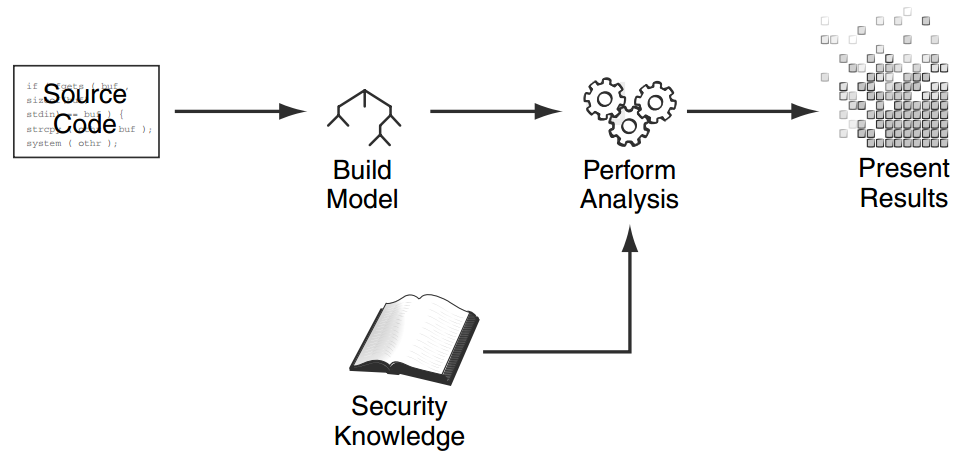
\includegraphics[width=1\linewidth]{img/analysis.png}
	\caption{Basic model of static code analysis \cite{Static_code_analysis_book_Chess:2007}}
	\label{fig:analysis}
\end{figure}

It is possible to differentiate two different kinds of analyses, lexical and data flow analysis.


\subsubsection{Lexical Analysis}
\label{subsec:lex_analysis}
The most analyzers do a form of lexical analysis.
They build a model like an AST with symbol tables, analyze nodes against specific rules and use pattern matching to find anomalies and bugs.
An early and easy example (2001) for such an analyzer is the Rough Auditing Tool for Security (RATS)\cite{Static_code_analysis_book_Chess:2007}, now acquired by the successful commercial tool Fortify\footnote{\href{http://www8.hp.com/de/de/software-solutions/application-security/}{Fortify: Static code analyzer by HP}}, that finds security and memory flaws in C source code, by doing a lexical analysis with XML-style rules, that contain already detailed descriptions of the corresponding problem.


\subsubsection{Dataflow Analysis}
\label{subsec:dataflow_analysis}
A data flow analysis uses additional models, like a \textit{Data Flow}- and \textit{Control Flow Graph (CFG)}, to find potential vulnerabilities and anomalies, by tracking data from inputs/sources to a leak/sink.
Typical analyses of that type are called Taint- or Live Variable Analysis.
The easiest kind of such an analyzer operates only in a single function body (\textit{intra-procedural}).
Depending on the desired goal, such an analysis can be \textit{flow-sensitive} (forward or top-down approach), to get control flow information about the past with more precision, or can be \textit{flow-insensitive} (backward or bottom-up approach), to get information about the future, but with less precision.


To extend the analysis scope to other functions, classes and packages (\textit{inter-procedural}), and automatically cover the different contexts (\textit{context-sensitivity}) of a whole program with variable aliases and other language features, additional models, like \textit{Call Graphs}, \textit{Point-To-Sets} and \textit{Inter-procedural Control Flow Graph's} are necessary.
Examples for sophisticated inter-procedural analyzers are Coverity\footnote{\href{https://www.coverity.com}{Coverity: Commercial inter-procedural static code analyzer}} and FlowDroid\footnote{\href{http://sseblog.ec-spride.de/tools/flowdroid}{FlowDroid: Context-, flow-, field-, object-sensitive and lifecycle-aware static taint analysis tool for Android applications}} from Eric Bodden at the TU Darmstadt.
With modern language features like reflection, virtual dispatch and multi-threading, static code analysis becomes more and more complex, hence the performance or precision decreases.


FindBugs and PMD implement a data flow analysis and they are the open source static analyzers we used later in our work for the evaluation.
Hence, they are described now.

\paragraph{PMD}
is a source code analyzer for Java, JavaScript, XML and XSL to find common programming flaws like unused variables, empty catch blocks, unnecessary object creation, etc.
It uses a set of rules, specified in a Java or XPath language, on an AST and control flow graph with data flow nodes to produce a report with rule violations in XML format.


\paragraph{FindBugs}
analyzes Java class files for programming defects and uses nearly 300 bug pattern with different categories (bad practice, correctness, etc.) and severity classes (high, medium and low)\cite{Findbugs}.
Unlike PMD, it is possible to write custom detectors in Java as plugins to analyze java-bytecode or source code.
The detectors use techniques like visitor patterns over class files, with state-machines to save types, stack-values, constants and other information and by traversing the control flow graph, to save conditional information.
The FindBugs detectors are usually not inter-procedural, but do an additional global analysis to know variable scopes and subtype-relationships.


Now it is important to distinguish when to apply analyzers in a Software Development Lifecycle.
Most analyzer, like FindBugs and PMD, exist as stand-alone version and allow the integration in common development tools, like IDE's, CI systems or Code Quality Management systems.




%\section{Input validation in popular frameworks}
%\label{sec:input_validation}
%\todo{Move this section to the end? - Brian}
%Check those \url{http://codegeekz.com/20-best-php-frameworks-developers-august-2014/} and make a table how input validation is handled there...
%The most common security weakness in any application is the failure to properly validate input from the environment. This weakness further leads to almost all of the major vulnerabilities in applications, including buffer overflow, SQL injection and a whole lot more. So, the maximum essential cautious measure that developers can take is to comprehensively authenticate the input that a software obtains. Certainly programs need to accept input, and computing a decent result depends on having a good input. There is a misconception that input can be trusted just because it is coming from some so-called trusted source. Input must not enter into the system without passing through various security methods.



\section{Static code analysis in IDE}
\label{sec:static_code_analysis_ide}
It is straightforward to integrate common analyzers like PMD and FindBugs in an Integrated Development Environment (IDE) like like Eclipse\footnote{An official list of Source Code Analysis plugins for Eclipse can be found in the \href{http://marketplace.eclipse.org/taxonomy/term/14,31}{Eclipse Marketplace}.}, Netbeans or IntelliJ.

With IDE (Integrated development environment), we mean a program ``that provides comprehensive facilities to computer programmers for software development. An IDE normally consists of a source code editor, build automation tools and a debugger.''\footnote{\href{http://en.wikipedia.org/wiki/Integrated_development_environment}{Integrated development environment}}
The IDE is usually the program that programmers use to develop new code, review code or fix bugs and issues. Since the programmer is used to navigate through the source using its IDE, it would be very helpful to enrich this environment by additional information. In contrast, reviewing analysis results in an independent and specialized program or website, code formatting and navigation can differ dramatically. Also, when it comes to fixing an issue, already being in the IDE means, a programmer can just make its changes instead of switching programs and locating the corresponding code location.

Static code analysis on IDE level is a common choice for many projects. Since the compile does many static analysis, it is effectively integrated into any IDE that can start the compile process and interprets that compilers output.

Advantages of integrating additional static code analyzers in IDEs:
\begin{itemize}
	\item Live feedback during programming
	\item Easy mapping of issues to code
	\item Possibility to fix issues early and instantly
	\item Reviewing and editing of source in one environment
	\item Interactive education for developers
	\item Extensibility thorough project specific rules
\end{itemize}

However disadvantages arise in bigger projects. Analyzers, especially data flow analyzers, tend to not to scale for big projects. 
There is no central way to configure the analyzer rules, to improve the results and performance.
Many developer tend to suppress warnings from such analyzers, since they produce a lot of false positives.
Hence, it is desired to have a central and independent analyzer, which can run on the remote repository code regularly and with predefined settings.

In this paper. we used the popular open source IDE Eclipse\footnote{\href{https://eclipse.org/}{https://eclipse.org/}}.
We decided for Eclipse because it is platform independent and highly extensible. Furthermore, we could integrate our test analyzers PMD and FindBugs into Eclipse. Therefore, the results are comparable with the other platforms we evaluated.


\section{Static code analysis in CI}
\label{sec:static_code_analysis_ci}
Continuous integration (CI) firstly proposed by Grady Booch \cite{CI-Definition:Booch:1993}, is the software engineering practice, of continuously merging all developer working copies with a shared release master branch several times a day.

Advantages and disadvantages of Continuous Integration (CI)\cite{SecurityinCI}:
\begin{itemize}
	\item[+] \textit{Immediate Notification}
	CI ensures that ongoing changes to the source code do not break the intent or design of the software. If a change does break the software, that break is identified immediately and can be fixed with a minimal cost and impact to the projects schedule.
	\item[+] \textit{Automated Testing and Deploying}
	CI enables many automation possibilities. The most useful automation area is testing in form of Unit- and Integration-Testing, to find problems after component integration and change introduced bugs in previously working components. 
	Finally a correct configured CI system can automate the deployment of software releases. 
	\item[+] \textit{Secure Development}
	By integrating security testing and secure code analysis, CI can be further leveraged to include secure development practices while minimizing the amount of extra effort required to get the benefits of secure development. Since it is tied to CI,
	security testing and secure code review begins when a project begins and runs continuously
	throughout project development. With CI, security vulnerabilities testing becomes part of the regression test bed, executed automatically with each successive build on the CI platform.
	
	\item[+] \textit{Changing Testing Economics}
	Using CI for build, test, and analysis automation has increased the depth and breadth of tests while also making them faster and less expensive. By making it cheap and easy to perform tests, teams are encouraged to test more and test sooner in the development cycle, reducing the cost of fixing bugs.
	
	\item[+] \textit{Trend and History}
	CI enables a higher management layer to view the history and trend of issues and builds.
	
	\item[-] \textit{CI Configuration}
	The configuration of a CI instance can be very troublesome and involves the understanding of many different tools. To create a working tool chain of testing, analyzing and building, with many thresholds and parameters the developer team has to understand every tool and have to tune parameters after gaining more experience.
\end{itemize}



\subsection{Levels of Integration}
Depending on how continuous integration is accomplished in a given process management, static code analysis can be performed at different \textit{locations}, times and with different automation and reporting levels. According to \cite[p. 6ff]{Jenkins:Smart:2011}, there are \textit{7 phases} of applying continuous integration to a specific development. For this overview, only 3 phases apply: \textit{Phase 1} there is no common build server, \textit{Phase 2} there is build server but builds run on a fixed (nightly) schedule and \textit{Phase 7} builds and tests (including analysis, measures) are issued as changes are committed.

\begin{itemize}
	\item[1] \textit{No Build Server} \\
	When no common build server exists, code analysis can only be applied on each developer's local machine. No developer is obliged to run the static code analysis before committing his changes nor will anybody be notified if code quality was decreased or new issues were introduced.
	
	
	\item[2] \textit{Nightly Builds} \\
	The build server could also run static code analysis and quality measures at each build and publish the results. Even notifications are possible, although they would not be accurately addressed since the system does not know which commit introduced the issue and can therefore not just notify the appropriate author.
	
	\item[3] \textit{Continuous Integration Environment} \\
	The server runs all test, analysis and code measures at each commit, publishes the results and notifies the appropriate developer when the build failed or new issues were introduced through his change.
\end{itemize}



\subsection{Jenkins}
\label{subsec:jenkins}
Jenkins is a widely used tool to control and manage continuous integration tasks. Its main purpose is to monitor the execution of repeated jobs and present their outcomes\footnote{From Jenkins Website, \href{https://wiki.jenkins-ci.org/display/JENKINS/Meet+Jenkins}{Meet Jenkins}}.

We decided for Jenkins because it is OpenSource, highly extensible and the most popular CI tool. To be exact, there are more than 1000 freely available plugins that can be installed by just one click using the Jenkins web interface.
Beside PMD and FindBugs, there are many more static analyzer available in the plugin repository.
In our research we found, almost every analyzer has a Jenkins plugin available.
Many OpenSource analyzers, like BrakeMan\footnote{\href{http://brakemanscanner.org/}{http://brakemanscanner.org/}}, Cppcheck\footnote{\href{http://cppcheck.sourceforge.net/}{http://cppcheck.sourceforge.net/}} as well as popular commercial tools like Coverity\footnote{\href{http://www.coverity.com/}{http://www.coverity.com/}} and Fortify\footnote{\href{http://www8.hp.com/de/de/software-solutions/application-security/}{http://www8.hp.com/de/de/software-solutions/application-security/}}.
But not all plugins provide a full analyzer.
Especially plugins for commercial tools like Coverity just provide a link to a corresponding web platform for code quality and issue management. 


%\begin{figure}[!t]
%	\centering
%	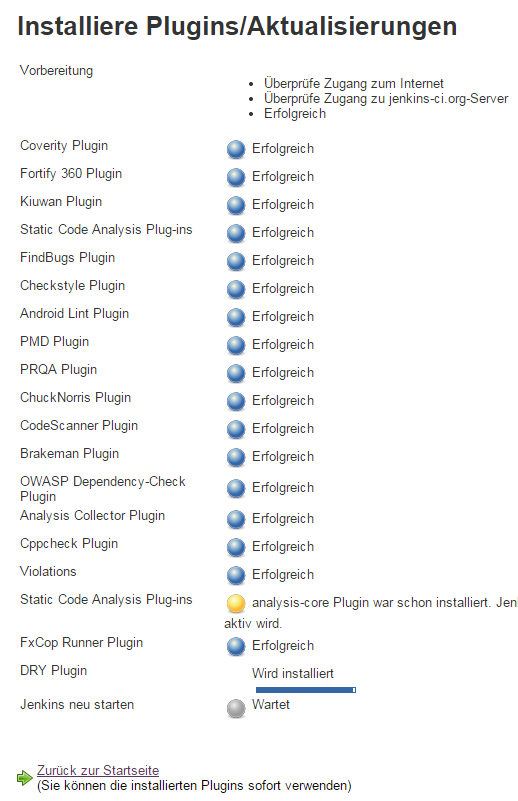
\includegraphics[width=1\linewidth]{img/jenkins-code-analysis-plugins.png}
%	\caption{Just a few used Jenkins plugins for static code analysis}
%	\label{fig:jenkins-plugins}
%\end{figure}


\subsection{Teamcity}
\label{subsec:static_code_analysis_teamcity}
Like Jenkins, Teamcity is a web application for continuous integration, published by the company Jetbrains\footnote{\href{https://www.jetbrains.com/teamcity/}{https://www.jetbrains.com/teamcity/}}. In contrast to Jenkins, its not open source, but freely available with a limitation of 20 build configurations.
Also it claims to be easier to use and configure than Jenkins.
It provides possibilities to run analyzers before or after the build process and to inspect resulting reports.
Furthermore it works together with static code analyzers in the commercial IntelliJ\footnote{\href{https://www.jetbrains.com/idea/}{https://www.jetbrains.com/idea/}} IDE from Jetbrains.

\begin{itemize}
	\item Installation: The Teamcity installation was a bit easier than Sonarqube because the database connection was configured in a wizard and similar it consists out of a webserver with webinterface (localhost:8111) and a database.
	
	\item Language support: All (since it is a highly customizable CI tool)
	
	\item Rule Management: The analyzers have to run externally and Teamcity will import the analysis results.
	Hence, it is much effort to configure and install different analyzers with different rulesets.
	
	\item Issue-Presentation: In the build details you can show issues in the Code Inspection tab, what present just the xml tree of the parsed reports, no filter options, no resolve options, no severity levels.
	
	\item Positive: Better user interface than Jenkins. With installed IDE plugin, you can jump to issue source-code directly in the IDE. 
	
	\item Negative: Hard to configure the external pmd and findbugs reports. Visualization of issues very limited. Two different inspections can not be processed during one build (skipped PMD report)
	
\end{itemize}



\section{Static code analysis in Code Quality Management}
\label{sec:static_code_analysis_code_quality_management}
\
\todo[inline]{Lofti: CQM although interesting, it is related to a different problem, unless you describe the connection to CI well.}

Code quality management (CQM) is the practice of monitoring and controlling the quality of code with different metrics and activities.
Static code analysis is a method of gaining measurements that can be used for CQM. Therefore, CQM tools can benefit at lot by a integration of static code analysis into a common build system.
\
\todo[inline]{quality management advantages and disadvantages}

\subsection{SonarQube}
\label{subsec:sonarqube}
SonarQube\footnote{\href{http://www.sonarqube.org/}{http://www.sonarqube.org/}} is an open source project, implemented as web application within its own webserver, with the aim to analyze and manage the quality of source code. 
Besides analysis against common coding guidelines, like duplicate code, missing comments and potential bugs, it also checks with an own rule engine (Squid) for several security issues (e.g. from the OWSASP Top 10 list).
Therefore it provides a central place to manage intuitively analysis rules from different analyzer extensions.
The main difference to CI tools, is the feature to manage the found issues.
Over plugins it is possible to extend the analysis scope to over 20 programming languages.


\begin{itemize}
\item Installation: SonarQube consists out of 3 parts: the local webserver (localhost:9000), a database to load and store analysis results and the sonarqube runner, which analyses the code specified in a project property file.

\item Language support: Java and other languages available as plugins

\item Rule Management: Very intuitive and easy to configure rules for so called quality profiles. Very interesting, that you can manage the rules of all analyzer plugins in one menu. It comes already with default sonarqube rules with different severity levels, detailed descriptions in different categories. Also including security relevant rules e.g. from OWASPTop10 and CWEs. One can compose a static analysis out of those rules including rules from plugins like FindBugs and PMD.

\item Issue-Presentation: Dashboard as starting point presents overview very well with different informative metrics, mostly for code quality and presents the number of issues of the different severity levels.
In the menu issues and issue-drilldown one can sort the issue list, search for issues matching to specific rules and get more information to the issue and most important where the issue is located in the code.

\item Positive: Good overview over issues, fast analysis, good rule management, good issue management with assigning issues to users etc.

\item Negative: In Rule-Management one can filter rules by tags and categories (bugs, security bugs), but you can not use those filters in the issue management. This leads to a big list of issues where you cant distinguish e.g. between a unused code and security issue.
 
\end{itemize}



\section{Evaluation}
\label{sec:evaluation}
We decided to make a qualitative evaluation, with usability inspection heuristics described in the book Information Visualization by Kerren et al. \cite{InformationVisualizationBook}.
From the work of Hollingsed et al. on 15 years of usability inspection evaluation \cite{15yearsUsabilityEvaluation}, we derived the best method would be a combination of a cognitive walk-through, combined with the usability heuristic evaluation defined by Nielsen \cite{Nielsen:UsabilityInspectionMethods}.
This wide-used, informal, very cost efficient and effective method is proven to find with a appropriate skilled evaluator team 55 - 90\% of all usability problems.


The usability inspection over heuristic evaluation method uses a small group of usability experts, who evaluate a
user interface using a set of guidelines and noting the severity of
each usability problem and where it exists. 
We combine it with a cognitive walk-though, in the way, that three experts go through the tools with a cognitive expected path in context of applying static code analysis with an additional usability guidelines list for every stage.


We identified four stages of our walk-through and evaluate several usability guidelines in each stage:


\subsection{Prepare analysis}
\begin{itemize}
	\item \textit{Is the tool easy and intuitive to configure?} \\
	In this category, we appraise how complicated it was, to set the continuous integration environment up and create a test project with our test source.
	
	\item \textit{Is it possible to add external analyzers?} \\
	This is a very useful feature, maybe even elementary. Not being able to add external analyzers means that only the included analyzers can be used.
	
	\item \textit{Is it possible to configure the analyzers?} \\
	Configuring static code analyzers is mandatory. For example, there is a huge trade of between accuracy and speed. Accurate analysis can result in very high computational costs. Keep in mind that the anaysis is supposed to run for each commit. If an analyzer run takes hours, this would not be practical anymore.
	
	\item \textit{Is it possible to view the rules?} \\
	This question targets the openness of the used static analysers. It can be very helpful to be able to view all supported rules if you want, for instance, check if a specific feature is checked or not. Additionally, viewing the rules can help to understand why an issue was reported and how the code can be improved.
	
	\item \textit{Is it possible to choose, add, edit, delete rules?} \\
	This is related to the previous question, but goes a little further. Imaging you got ascertain that at specific flaw is not detected by a static code analyser. In case, the analyser supports the editing of the used ruleset, you can simply add a custom rule or edit an existing one.
	
	Choosing (selecting) only a subset of all existing rules can result in a faster analyser run which can come in very handy if frequent analyzis should be performed, e.g. at each commit and thereby multiple times a day.
\end{itemize}


\subsection{Run analysis}
\begin{itemize}
	\item \textit{Is it easy and intuitive to start the analysis?} \\
	How much effort is required to manually start an analysis? Is this even possible or are only automated analysis supported? Furthermore, starting an anylsis can be easy as a click on a website or hard like a manuell invokation of a specific command on the source code folder on some server.
	
	\item \textit{Is it possible to following the analysis progress?} \\
	This can be useful if an anylsis takes some time and the process cannot be determinded in a different way. Also, the analyser output can be helpful for debugging purposes.
\end{itemize}


\subsection{Evaluate analysis results}
\begin{itemize}
	\item \textit{Is there an issue overview with severity levels?} \\
	\item \textit{Is it possible to view an issue trend/history?} \\
	\item \textit{Is there a mapping from issue to source code position?} \\
	\item \textit{Is there a description for every issue?} \\
	\item \textit{Is the issue description easy to understand with solution suggestions?} \\
	\item \textit{Is there a possibility to filter issues? (severity, category, tag, ...)} \\
\end{itemize}


\subsection{Manage analysis results}
\begin{itemize}
	\item \textit{Is it possible to assign issues to developers?} \\
	\item \textit{Is is possible to edit issue status? (Resolved, False positive, ...)} \\
\end{itemize}



\subsection{Eclipse}
\label{subsec:evaluation_eclipse}

\subsection{Jenkins}
\label{subsec:evaluation_jenkins}

\begin{figure}[t]
	\centering
	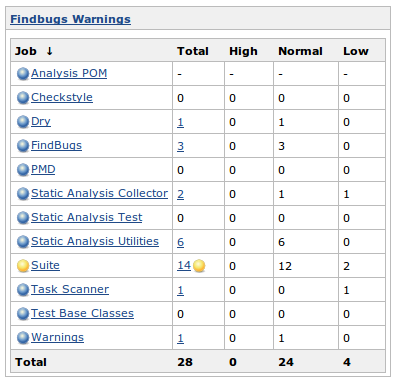
\includegraphics[width=0.45\textwidth]{img/jenkins_dashboard.png}
	\caption{Jenkins Dashboard using the common ``Static Code Analysis Plug-ins'' plugin that combines the results of multiple analyzers.}
	\label{fig:jenkins-dashboard}
\end{figure}

Jenkins itself has no static code analysis included but a major feature of Jenkins is its extensibility. Including a code analysis step in a build process is simple as adding a \textit{build step}. The analyzers configuration can be passed by command line options or via a configuration file, depending on the used analyzer. How well an analyzer can be configured or if the ruleset can be modified depends not on Jenkins but only on the analyzer. We can, therefore, make no statement about this.

Starting an analysis in Jenkins is easy as pressing the respective button in the web interface. The process can be watched live in a self-reloading page that prints all console output that is made by all build steps. Since static code analysis is just a build step in Jenkins, the output of the analyzers is visible there too.

Visualization of analysis results is done by free plugins only. In general, the analyzer creates a result file that is written to a specific location. After the build is done, the relevant plugins check the project root for those result files and parse their content. Therefore, the way the results are shown depends largely on the quality of the used plugin. Nevertheless, one common static code analyzis plugin exists\footnote{\href{https://wiki.jenkins-ci.org/display/JENKINS/Static+Code+Analysis+Plug-ins}{Jenkins: Static Code Analysis Plug-ins}}, that is able to collect the results of multiple plugins and create a common overview over all results, see figure \ref{fig:jenkins-dashboard}. Again, the quality of this visualizations depends hardly on the quality of the available plugins for a specific analyzer. We observed a good support and an ordinary visualization quality but these information is only founded on samples.




\subsection{Teamcity}
\label{subsec:evaluation_teamcity}

\subsection{SonarQube}
\label{subsec:evaluation_sonarqube}


\subsection{Comparison}
\label{subsec:comparation}

\begin{figure*}[t]
	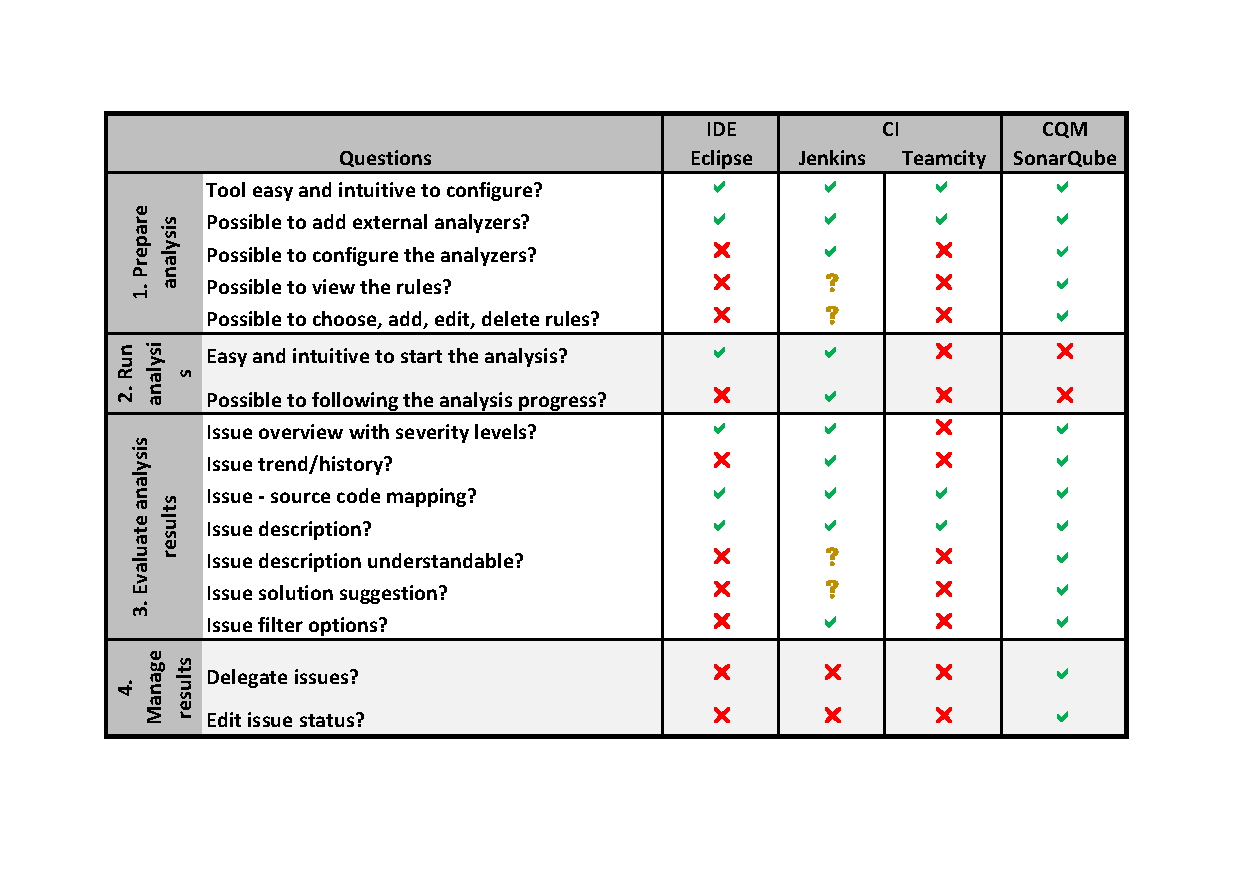
\includegraphics[width=\textwidth]{img/comparation}
	\caption{Comparison Matrix.}
	\label{fig:comparison_matrix}
\end{figure*}


\todo[inline]{Describe the final analysis results (matrix)}

\section{Conclusion}
\label{sec:conclusion}
\begin{itemize}
	%\item Conclusion about how input validation is done in frameworks, what can be better ...
	\item Its really not that easy to find the right static code analyzer for your project with a specific programming language. There are lots of open source tools, but very old and just supported by Jenkins over hacks.
	\item static code analyzer need to be customized to find special problems (like Java Vulnerabilities)
	\item Is it better to integrate static analysis in Jenkins or in IDE or in Code Quality Management tools?
	\item Is reporting in Jenkins useable? No...just in combination with code quality management tools like SonarQube, Coverity, ... and the analysis in those tools can be triggered in CI tools, but it is much effort to configure.
	\item Future work: Using many tools is basically a good idea, because more tools find potentially more vulnerabilities. A future approach would be to implement a tool that can filter all the generated reports. Thereby duplicate vulnerabilities findings can be merged and false positives can be reduced.
\end{itemize}



\bibliographystyle{IEEEtran}
% argument is your BibTeX string definitions and bibliography database(s)
\bibliography{references}

\end{document}


